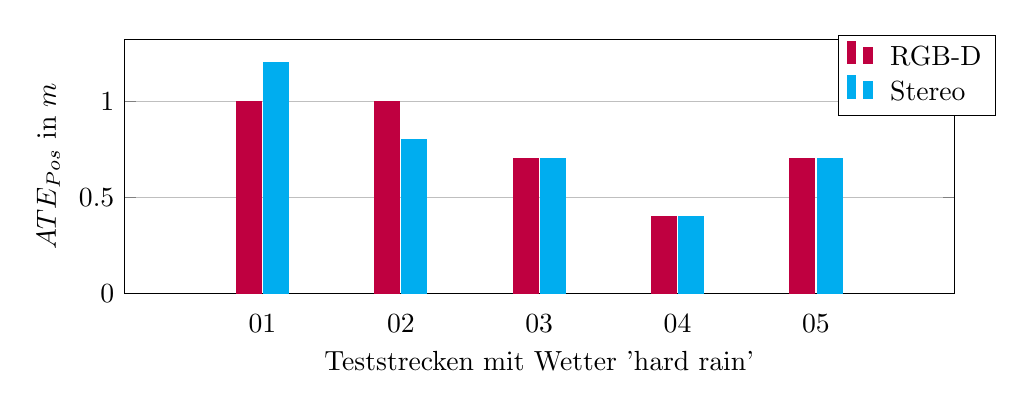
\begin{tikzpicture}
    \begin{axis}[
        width  = \textwidth,
        height = 4.8cm,
        major x tick style = transparent,
        ybar=2*\pgflinewidth,
        bar width=9pt,
        ymajorgrids = true,
        ylabel = {$ATE_{Pos}$ in $m$},
        xlabel = {Teststrecken mit Wetter 'hard rain'},
        symbolic x coords={01, 02, 03, 04 ,05},
        xtick = data,
        scaled y ticks = false,
        enlarge x limits=0.25,
        ymin=0,
        legend cell align=left,
        legend style={
                at={(1.05,.7)},
                anchor=south east,
                column sep=1ex
        }
    ]
        \addplot[style={purple,fill=purple,mark=none}]
            coordinates {(01, 1.0) (02,1.0) (03, .7) (04 ,.4) (05, .7)};
  
        \addplot[style={cyan,fill=cyan,mark=none}]
            coordinates {(01, 1.2) (02,.8) (03, .7) (04 ,.4) (05, .7)};
  
        \legend{RGB-D, Stereo}
    \end{axis}
  \end{tikzpicture}